%%%%%%%%%%%%%%%%%%%%%%%%%%%%%%%%%%%%%%%%%%%%%%%%%%%%%%%%%%%%%%%%%%%%%%%%%%%%%%%
%%%%%%%%%%%%%%%%%%%%%%%%%%%%%%%%%%%%%%%%%%%%%%%%%%%%%%%%%%%%%%%%%%%%%%%%%%%%%%%
%%
%%
%%             b.   M  E  T  H  O  D  O  L  O  G  Y  
%%
%%
%%%%%%%%%%%%%%%%%%%%%%%%%%%%%%%%%%%%%%%%%%%%%%%%%%%%%%%%%%%%%%%%%%%%%%%%%%%%%%%
%%%%%%%%%%%%%%%%%%%%%%%%%%%%%%%%%%%%%%%%%%%%%%%%%%%%%%%%%%%%%%%%%%%%%%%%%%%%%%%

%% http://hubblesite.org/image/2012/news_release/2006-51
\section{Methodology}
\noindent
This ERC Consolidator proposal kick starts the new field of Variable
Extragalactic Astrophysics. Due to the Data Science aspect of this
proposal, it is, at its heart interdisciplinary.  We present a bold
research vision that is designed to be addressed by a research group,
and the environment, current research areas and telescope access at
the Institute for Astronomy at the University of Edinburgh is ideal to
carry out these investigations.  


\smallskip
\smallskip
\noindent
In this section, we first introduce the missions, surveys and novel
instrumentation that will be the experimental backbone of this
proposal. In Table 1, we state in detail our objectives and tie
them to the datasets and novel investigations we plan in our Work Packages
(WPs).  We then describe our approach to building our core data
science infrastructure while breaking down the data silos. We give more
details for each WP and conclude this section with a Feasibility
report.


\subsection{Upcoming Surveys, Instruments and Missions}
\noindent
\citep{Lawrence2016_ASPC} emphasize that variability studies hold
information on otherwise unresolvable regions in quasars. Likewise,
population studies of large samples likewise have been very productive
for our understanding of quasars. These two themes are coming together
in the idea of systematic variability studies of large samples and
{\it over the next 5 or so years} the field of observational
extragalactic astrophysics is poised for a fundamental and rapid
change.

\smallskip
\smallskip
\noindent
Starting in late 2019, a fleet of new telescopes, instruments and
missions are coming online over the next few years that will leap-frog
the quality and quantity of data we have available today. Over the
course of the next 5-6 years, surveys and missions including the fifth
incarnation of the Sloan Digital Sky Survey
(SDSS-V\footnote{\href{www.sdss.org/future/}{{\tt
www.sdss.org/future/}}}), the Large Synoptic Survey Telescope
(LSST\footnote{\href{lsst.org}{{\tt lsst.org}}}), the Dark Energy
Spectroscopic Instrument (DESI\footnote{\href{desi.lbl.gov}{{\tt
desi.lbl.gov}}}) survey, the 4-meter Multi-Object Spectroscopic
Telescope (4MOST\footnote{\href{4most.eu}{{\tt 4most.eu}}}) survey,
and the ESA {\it Euclid}
mission\footnote{\href{sci.esa.int/euclid/}{{\tt
sci.esa.int/euclid/}}}, will see first light. Even more imminent is
the launch of the {\it James Webb Space Telescope}
(JWST\footnote{\href{jwst.stsci.edu}{{\tt jwst.stsci.edu}}}).

%
\begin{framed}
 \begin{tcolorbox}
   \begin{center} 
     Overview of Facilities and Surveys related to this proposal
   \end{center}
 \end{tcolorbox}
  
\noindent
\textbf{\textsc{Imminent:}}

The {\bf Sloan Digital Sky Survey (SDSS):} An ongoing project,
currently in its fourth phase, SDSS-IV.  {\bf The P.I. was a leading
member of the SDSS-III: Baryon Oscillation Spectroscopic Survey (BOSS;
see Track Record and C.V.).} The fifth generation of Sloan Digital Sky
Surveys, SDSS-V will be an all-sky, multi-epoch spectroscopic survey,
yielding spectra of over 6 million objects during its lifetime. In
particular, the SDSS-V Black Hole Mapper (BHM) will focus on
long-term, time-domain studies of AGN, including direct measurement of
black hole masses and changing-look quasars, and on the optical
characterization of eROSITA X-ray sources. Data taking is due to start
in 2020. Access would be through a \euro184,100 `buy-in', which allows
access for the P.I. and one PDRA.  {\it Data Products: Repeat spectra
in the North and Southern Hemisphere for 500,000 bright QSOs.} \\

The {\bf Dark Energy Spectroscopic Instrument (DESI) Survey:} is a 5
year cosmology survey that will be conducted on the Mayall 4-meter
telescope at Kitt Peak National Observatory starting in 2019. It uses
the 5,000 fiber Dark Energy Spectroscopic Instrument and will obtain
optical spectra for $\approx$20 million galaxies and quasars.  {\bf
The P.I. helped write the original science case and proposal for DESI
\citep{Schlegel2011} but having left the U.S./LBNL, no longer has data
access rights.}  The DESI Survey starts in late 2019 and data access
is through a \euro200,100 `buy-in', which allows access for the
P.I. and two PDRAs.  {\it Data Products: Spectra of 1e6 quasars across
14,000 deg$^{2}$ of the Northern Sky.} \\

The {\bf Large Synoptic Survey Telescope (LSST)} project will conduct
a 10-year survey of the sky, imaging the full Southern Sky every 3
nights. The LSST survey is designed to address four science areas
(Understanding the Mysterious Dark Matter and Dark Energy; Hazardous
Asteroids and the Remote Solar System; The Transient Optical Sky; The
Formation and Structure of the Milky Way) and is an absolutely unique
facility as far as areal, temporal and wavelength coverage. The U.K.
is a member of LSST.  {\it Data Products: $ugrizY$ broadband optical
and near-infrared imaging for 20,000 deg$^2$.  Images the full
Southern Sky every 3 days.} \\

\textit{\textbf{Euclid}} is an ESA Medium Class mission to map the
geometry of the dark Universe.  It aims to understand why the
expansion of the Universe is accelerating and what the nature of the
source responsible for this acceleration (``dark energy'') is.  The
mission will investigate the distance-redshift relationship and the
evolution of cosmic structures by measuring shapes and redshifts of
galaxies and clusters of galaxies out to redshifts $\sim$2, or
equivalently to a look-back time of 10 billion years. {\it Euclid} will 
also discover a range of near-infrared (NIR) detected quasars,  
 {\it Euclid} is planned for launch in mid-2021.  {\it Data Products: Very broadband
optical and 3 filter near-infrared space-based imaging for 15,000
deg$^2$.} \\

The {\bf 4-metre Multi-Object Spectroscopic Telescope (4MOST):} is a
fibre-fed spectroscopic survey facility on the VISTA telescope with a
large enough field-of-view to survey a large fraction of the southern
sky. The facility will be able to simultaneously obtain spectra of
2,400 objects distributed over a field-of-view of 4 square degrees.
The initial Galactic and Extragalactic surveys will operate over a
five-year period delivering spectra for $\geq$25 million objects over
$\gtrsim$15,000 deg. 4MOST will commence science operations in early
2022. {\it Data Products: } 5MOST will operate continuously for an
initial five-year public survey delivering spectra for $\geq$25
million object over 15,000 deg$^{2}$.\\

The {\bf James Webb Space Telescope (JWST)} is a space telescope
developed in coordination among NASA, the European Space Agency, and
the Canadian Space Agency. It is scheduled to be launched in June
2019. The telescope will offer unprecedented resolution and
sensitivity from 0.6 to 27$\mu$m. JWST is a partnership between NASA,
ESA and the Canadian Space Agency.  In particular, ESA's contributions
to JWST include (but are not limited to) the NIRSpec instrument and
the Optical Bench Assembly of the MIRI instrument.  In return for
these contributions, ESA gains full partnership in JWST and secures
full access to the JWST observatory for astronomers from ESA Member
States on identical terms to those of today on the {\it Hubble Space
Telescope}. {\it Data Products: Revolutionary optical to mid-infrared
deep-field imaging and spectra.  Unique access to wavelengths
$\lambda>2\mu$m, inaccessible from the ground, ideal for high-$z$
quasar studies.} \\


The {\bf Extended Roentgen Survey with an Imaging Telescope Array
(eROSITA)} is the main instrument on the Spektr-RG mission, an
international high-energy astrophysics observatory.  Set to launch in
2019 with both high sensitivity and a large FOV, eROSITA will discover
as many new X-ray sources in its first twelve months as are known
today, after more than 50 years of X-ray astronomy.  SDSS-V will
provide optical spectroscopic measurements including identifications
and redshifts, of $\sim$400,000 eROSITA X-ray sources detected in the
first 1.5 years of the all sky survey.  In addition, SDSS-V's BHM will
characterize numerous serendipitous discoveries, extreme and rare
objects, transients, and other peculiar variables found in the eROSITA
survey \citep{Merloni2012}, and expand an optical+X-ray quasar sample
with implications for observational cosmological constraints
\citep[e.g.][]{Risaliti_Lusso2015}.\\

\underline{Notes:} 4MOST has full access to the full LSST
footprint. LSST will overlap half (7,500 deg$^2$) of the {\it Euclid}
footprint. Data access to eROSITA sources is via an MOU with  
SDSS-V. \\

\hrulefill 

\noindent
\textbf{\textsc{Ongoing:}} 

The {\bf Wide-field Infrared Survey Explorer (WISE)} is a NASA
infrared-wavelength astronomical space telescope launched in December
2009 and is still operation (as at the time of writing, in its
``NEOWISE-R'' mission phase). WISE performed an all-sky astronomical
survey with images at 3.4, 4.6, 12 and 22$\mu$m using a 40cm (16 in)
diameter infrared telescope in Earth orbit.  {\bf The P.I. is a world
expert in quasar identification using WISE \citep[e.g., ][]{Ross2012,
Ross2015, Timlin2016, Timlin2018} and exploiting mid-infrared light
curve data.} \\

The \textbf{ESA {\it Gaia}} mission is an ongoing mission to chart a
three-dimensional map of our Galaxy, the Milky Way, in the process
revealing the composition, formation and evolution of the Galaxy. Gaia
is providing unprecedented positional and radial velocity measurements
with the accuracies needed to produce a stereoscopic and kinematic
census of about $\sim$one billion stars in our Galaxy and throughout
the Local Group. This amounts to about 1 per cent of the Galactic
stellar population.
\end{framed}


\begin{framed}
 \begin{tcolorbox}
   \begin{center} 
     Overview of Facilities and Surveys related to this proposal
   \end{center}
 \end{tcolorbox}
  
\noindent
\textbf{\textsc{Imminent:}}

The {\bf Sloan Digital Sky Survey (SDSS):} An ongoing project,
currently in its fourth phase, SDSS-IV.  {\bf The PI was a leading
member of the SDSS-III: Baryon Oscillation Spectroscopic Survey (BOSS;
see Track Record and C.V.).} The fifth generation of Sloan Digital Sky
Surveys, SDSS-V will be an all-sky, multi-epoch spectroscopic survey,
yielding spectra of over 6 million objects during its lifetime. In
particular, the SDSS-V Black Hole Mapper (BHM) will focus on
long-term, time-domain studies of AGN, including direct measurement of
black hole masses and Changing-Look quasars, and the optical
characterization of eROSITA X-ray sources. Data taking for SDSS-V is due to start
in 2020.  {\it Data Products: Multiple repeat spectra
in the North and Southern Hemisphere for 500,000 quasars.} \\

The {\bf Dark Energy Spectroscopic Instrument (DESI) Survey} is a 5
year cosmology survey that will be conducted on the Mayall 4-meter
telescope at Kitt Peak National Observatory starting in late 2019. It uses
the 5,000 fiber Dark Energy Spectroscopic Instrument and will obtain
optical spectra for $\approx$20 million galaxies and quasars.  {\bf
The PI contributed in writing the original science case and proposal
for DESI \citep{Schlegel2011} but having left the U.S./LBNL, he no
longer has data access rights.}  {\it Data Products: Spectra of 1e6
quasars across 14,000 deg$^{2}$ of the Northern Sky.} \\

The {\bf Large Synoptic Survey Telescope (LSST)} project starts data
taking in late 2021, and will conduct a full survey of the
Southern Sky every 3 nights. The LSST survey is designed to address
four science areas (Understanding Dark Matter and Dark
Energy; Hazardous Asteroids and the Remote Solar System; The Transient
Optical Sky; The Formation and Structure of the Milky Way) and is an
absolutely unique facility as far as areal, temporal and wavelength
coverage. The U.K.  is a member of LSST giving me free data access
rights (to the raw, unfiltered data).  {\it Data Products:
$ugrizY$ broadband optical and near-infrared imaging for 20,000
deg$^2$.  Images the full Southern Sky every 3 days.} \\
%% LSST:: Each patch of sky it images will be visited 1000 times during the survey,


\textit{\textbf{Euclid}} is an ESA Medium Class mission due for launch
in mid-2021 that will map the geometry of the dark Universe.  It aims
to understand why the expansion of the Universe is accelerating and
what the nature of the source responsible for this acceleration
(``dark energy'') is.  The mission will investigate the
distance-redshift relationship and the evolution of cosmic structures
by measuring shapes and redshifts of galaxies and clusters of galaxies
out to redshifts $\sim$2, or equivalently to a look-back time of 10
billion years. {\it Euclid} will also discover a range of
near-infrared (NIR) detected quasars, {\it Euclid} is planned for
launch in mid-2021.  {\it Data Products: Very broadband optical and 3
filter near-infrared space-based imaging for 15,000 deg$^2$, 
overlapping SDSS-V in the North and LSST in the South.} \\

The {\bf 4-metre Multi-Object Spectroscopic Telescope (4MOST):} is a
fibre-fed spectroscopic survey facility on the VISTA telescope with a
large field-of-view in order to survey a large fraction of the Southern
sky. The facility will be able to simultaneously obtain spectra of
2,400 objects distributed over a field-of-view of 4 deg$^{2}$.
The initial Galactic and Extragalactic surveys will operate over a
five-year period delivering spectra for $\geq$25 million objects over
$\gtrsim$15,000 deg$^{2}$. 4MOST will commence science operations in early
2022. {\it Data Products: } 4MOST will operate continuously for an
initial five-year public survey delivering spectra for $\geq$25
million object over 15,000 deg$^{2}$.\\

The \textbf{\emph{James Webb Space Telescope} (JWST)} is a space
telescope developed in coordination among NASA, ESA and the Canadian
Space Agency. It is scheduled to be launched in June 2019. The
telescope will offer unprecedented resolution and sensitivity from 0.6
to 27$\mu$m. ESA's contributions to JWST include (but are not limited
to) the NIRSpec instrument and the Optical Bench Assembly of the MIRI
instrument.  In return for these contributions, ESA gains full
partnership in JWST and secures full access to the JWST observatory
for astronomers from ESA Member States. {\it Data Products:}
Revolutionary optical to mid-infrared deep-field imaging and spectra.
Unique access to wavelengths $\lambda>2\mu$m, inaccessible from the
ground, ideal for high-$z$ quasar studies. \\


The {\bf Extended Roentgen Survey with an Imaging Telescope Array
(eROSITA)} is the main instrument on the Spektr-RG mission, an
international high-energy astrophysics observatory.  Set to launch in
2019 with both high sensitivity and a large FOV, eROSITA will discover
as many new X-ray sources in its first twelve months as are known
today, after more than 50 years of X-ray astronomy.  SDSS-V will
provide optical spectroscopic measurements including identifications
and redshifts, of $\sim$400,000 eROSITA X-ray sources detected in the
first 1.5 years of the all sky survey.  In addition, SDSS-V's BHM will
characterize numerous serendipitous discoveries, extreme and rare
objects, transients, and other peculiar variables found in the eROSITA
survey \citep{Merloni2012}, and expand an optical+X-ray quasar sample
with implications for observational cosmological constraints
\citep[e.g.][]{Risaliti_Lusso2015}.\\

%\underline{Notes:} 4MOST has full access to the full LSST footprint. LSST will overlap half (7,500 deg$^2$) of the {\it Euclid} footprint. Data access to eROSITA sources is via an MOU with SDSS-V. \\
%\hrulefill 

\noindent
\textbf{\textsc{Ongoing:}} 

The {\bf Wide-field Infrared Survey Explorer (WISE)} is a NASA
infrared-wavelength astronomical space telescope launched in December
2009 and is still operation (as at the time of writing, in its
``NEOWISE-R'' mission phase). WISE performed an all-sky astronomical
survey with images at 3.4, 4.6, 12 and 22$\mu$m using a 40cm (16 in)
diameter infrared telescope in Earth orbit.  {\bf The P.I. is a world
expert in quasar identification using WISE \citep[e.g., ][]{Ross2012,
Ross2015, Timlin2016, Timlin2018} and exploiting mid-infrared light
curve data.} \\

The \textbf{ESA {\it Gaia}} mission is an ongoing mission to map 
the Milky Way in three-dimensions, in the process
revealing the composition, formation and evolution of the Galaxy. {\it Gaia} 
is providing unprecedented positional and radial velocity measurements
with the accuracies needed to produce a stereoscopic and kinematic
census of about $\sim$one billion stars in our Galaxy and throughout
the Local Group. This amounts to about 1 per cent of the Galactic
stellar population.

\end{framed}


\begin{framed}
 

\noindent
\textbf{\textsc{Ongoing:}} 

The {\bf Wide-field Infrared Survey Explorer (WISE)} is a NASA
infrared-wavelength astronomical space telescope launched in December
2009 and is still operation (as at the time of writing, in its
``NEOWISE-R'' mission phase). WISE performed an all-sky astronomical
survey with images at 3.4, 4.6, 12 and 22$\mu$m using a 40cm (16 in)
diameter infrared telescope in Earth orbit.  {\bf The P.I. is a world
expert in quasar identification using WISE \citep[e.g., ][]{Ross2012,
Ross2015, Timlin2016, Timlin2018} and exploiting mid-infrared light
curve data.} \\

The \textbf{ESA {\emph Gaia}} mission is an ongoing mission to chart a
three-dimensional map the Milky Way, in the process
revealing the composition, formation and evolution of the Galaxy. 
Gaia
is providing unprecedented positional and radial velocity measurements
with the accuracies needed to produce a stereoscopic and kinematic
census of about $\sim$one billion stars in our Galaxy and throughout
the Local Group. 
%This amounts to about 1 per cent of the Galactic stellar population.

\end{framed}



\smallskip
\smallskip
\noindent
%%%%%%%%%%%%%%%%%%%%%%%%%%%%%%%%%%%%%%%%%%%%%%%%%%%%%%%%%%%%%%%%%%%%%%%%%%%%%%%%
%%
%%  https://tex.stackexchange.com/questions/337820/mcq-long-table-using-tikz-tcolorbox-or-tabular
%%  https://tex.stackexchange.com/questions/283419/color-in-a-multirow-cell-with-extra-vertical-space/283454
%%  https://tex.stackexchange.com/questions/406033/how-to-fit-a-cell-of-a-table-to-a-figure-and-arrange-multiple-tables/406042
%% 
%% THIS (??)::
%%     https://texblog.org/2014/05/19/coloring-multi-row-tables-in-latex/
%%
%%
%%   https://www.inf.ethz.ch/personal/markusp/teaching/guides/guide-tables.pdf
%%
%%%%%%%%%%%%%%%%%%%%%%%%%%%%%%%%%%%%%%%%%%%%%%%%%%%%%%%%%%%%%%%%%%%%%%%%%%%%%%%%


\begin{tcolorbox}[tab1, tabularx={X  X }, title=Outstanding Issues in Extragalactic Astrophysics, boxrule=1.25pt] 
Key issue                                                                            &  Novel investigation       \\ 
\hline \hline
\multicolumn{2}{c}{{\sc The physics of accretion}} \\ 
Investigating ``hot'' and ``cold'' mode accretion in the quasar population; 
determining the rates and timescales, and characterising the Changing Look Quasar (CLQ) population.   &     
Identifying and characterizing  all the CLQs in DESI and SDSS-V.  \\ 
\hline
Probing the inner parsec of the quasar central engine & 
Rapid analysis and response on LSST quasar light curves. \\ 
\hline
%%
\multicolumn{2}{c}{{\sc Obscured accretion and galaxy formation}} \\
Establish the relative importance of major mergers, minor mergers, cold streams and secular evolution 
have towards the growth of SMBHs across cosmic time. & 
Deep imaging data from LSST combined with searching for post-starburst signatures 
in DESI, SDSS-V, 4MOST spectra. NIRcam and MIRI imaging from JWST. \\ \hline
Establishing the bolometric output and origin of IR emission, and  
determine presence of extreme outflows in the $z\sim2-3$ quasar population. & 
MIRI MRS spectroscopy with JWST.\\ \hline
Establishing the range of SED parameter space the quasars occupy by a multi-wavelength multi-epoch ``truth table dataset'' & 
Building ``The Stripe 82 Rosetta Stone'' (SpIES, SHELA, VICS82, S82X, HSC; repeat optical observations from SDSS, DES) \\ \hline
%%
Find the physical conditions under which SMBH grew at the epoch when most of the accretion and star formation in the Universe occurred ($z\sim1-4$) & Perform a complete census of AGN across $z\sim0-7$, focussing on $z=1-4$ using medium-deep multiwavelength datasets \\ \hline
\multicolumn{2}{c}{{\sc Galaxy-scale feedback}}\\
Establishing the theoretical impact of extreme outflows in the $z\sim2-3$ quasar population & 
Hydro simulation modelling.  \\
\hline
Understand how the accretion disks around black holes launch winds and outflows and determine how much energy these carry. 
Quantify the amount of ``Maintenance/Jet/Kinetic'' mode and ``Transition/Radiative/Wind'' mode feedback.
& 
Identifying and characterizing  all the CLQs in DESI and SDSS-V.  \\ 
    %\end{tcbitemize}
\end{tcolorbox}



\subsection{Data Science and Data Silos}
\smallskip
\smallskip
\noindent
\textbf{\textsc{{Data Science and Observational Astrophysics: }}}
Data science is a new interdisciplinary field of scientific methods to
extract knowledge or insights from data in various forms, either
structured or unstructured. It employs techniques and theories drawn
from many fields within the broad areas of mathematics, statistics,
information science, and computer science, in particular from the
subdomains of machine learning, classification, cluster analysis, data
mining, databases, and visualization.  {\it Modern day observational
astrophysicists are in all but name data scientists, and as such, this
proposal is inherently interdisciplinary.}

\smallskip
\smallskip
\noindent
\textbf{\textsc{Breaking Down The Data Silos: }}
The bottleneck to using advanced data analysis is not skill base or
technology; it is simply access to the data.  A data silo is a
repository of fixed data that remains under the control of one
department/collaboration and is isolated from the rest of the world,
much like grain in a farm silo is closed off from outside
elements. These silos are isolated islands of data, and they make it
prohibitive to extract data and put it to other uses. In research
environments, and especially in contemporary observational
astrophysics, the data silos are open, but due to the lack of raw
person-power, still remain uncombined. {\it The combination of P.I. and
host institute means we are uniquely positioned to break down these
astro-data silos for massively significant science gain.}



\smallskip
\smallskip
\noindent
\textbf{\textsc{Targeting Big Data: }}
This ERC will develop and employ leadership-computing systems and
infrastructure to explore, prove, and improve a wide range of data
science techniques: uncertainty quantification; statistics; machine
learning; deep learning; databases; pattern recognition; image
processing; graph analytics; data mining; real-time data analysis; and
complex and interactive workflows.

\smallskip
\smallskip
\noindent
\textbf{\textsc{Algorithms: }}
Our algorithms and methodology are based on the latest
machine-learning and data science techniques. Specifically we will use
\href{https://www.python.org/}{Python} as the CS-glue,
\href{http://www.numpy.org/}{NumPy} for high-speed numerical
processing, \href{https://pandas.pydata.org/}{pandas} for efficient
data ingestion and \href{https://matplotlib.org/}{Matplotlib} for data
visualization.  The \href{http://www.astropy.org/}{Astropy Project} is a
community effort to develop a common core package for Astronomy in
Python and foster an ecosystem of interoperable astronomy packages,
and one the P.I. and his team fully use and support.
%%
\href{http://ogrisel.github.io/scikit-learn.org/sklearn-tutorial/index.html}{\tt
scikit-learn} is a Python module integrating classic machine learning
algorithms in the scientific Python world. It aims to provide simple and efficient solutions to
learning problems, accessible to everybody and reusable in various
contexts. Resources such as the
\href{https://github.com/jakevdp/PythonDataScienceHandbook}{{\tt
Python Data Science Handbook}} have full details. 
%This includes the ``extreme deconvolution'' \href{http://www.sdss.org/dr14/data\_access/value-added-catalogs/?vac\_id=xdqso/}{`XDQSO' technique}\footnote{\href{https://github.com/xdqso/xdqso}{\tt github.com/xdqso/xdqso}}.
These are the solid foundations on which we intended to build our software packages, 
including {\tt QuasarSieve}. 
{\bf We nota bene that the P.I. and his research group has a strong track 
record of building, combining and utilizing new ML algorithms for 
quasar science e.g., \citet{Ross2012}.}




\smallskip
\smallskip
\noindent
\textbf{\textsc{Open Innovation, Open Science, Open to the World:}}
The P.I. is an exceptionally strong, longtime and vocal supporter of
``Open Access''.  All my codes, data\footnote{Where I am not breaking
current data access agreements}, papers and proposals can be found at
\href{github.com/d80b2t}{{\tt github.com/d80b2t}}.  Indeed, this
proposal itself is now at that location.  One of the major research
outputs of this ERC will be computer code.  As such, we are already
working with the \href{\tt https://www.software.ac.uk/}{The Software
Sustainability Institute} which was founded to support the UK's
research software community.  Our software well be developed using the
FAIR ideology (Findable, Accessible, Interoperable,
Reusable\footnote{Wilkinson, MD, Sci Data. 2016 Mar 15;3:160018. doi:
10.1038/sdata.2016.18.})  and will be delivered in a manner which is
fully inline with ``Open Innovation, Open Science, Open to the
World''.

\begin{figure}
  \begin{center}
   \hspace{-0.5cm}
%   trim=l b r t
    \includegraphics[width=16.0cm, trim={0.25cm 7.0cm 0.25cm 1.0cm},clip]
%    {figures/WP_overview_wEuclid.pdf}
    {figures/WP_overview_landscape_rounded.pdf}
    \vspace{-10pt}
    \caption{An overview of our WPs. Arrows give general data or
      workflow, though natural iteration is expect, accounted and not
      necessarily shown. Asterisks show lead PDRA where necessary. $\Phi$
      indicative of giving quasar space density, see e.g., \citet{Ross2013}.
      $S_{i,j}$ indicative of a model for the time variability of quasars as
      a stochastic process described by the exponential covariance matrix
      \citep[see e.g.,][]{MacLeod2010}.}
    \vspace{-12pt}
 \label{fig:workplan}
\end{center}
\end{figure}


\subsection{Work Packages}
%\smallskip \smallskip \noindent {\bf  WORK  $\;$  PACKAGES} 
\smallskip 
\smallskip
\noindent
Our proposal contains six work packages that fall into three broad and
complementary categories: observational studies of large numbers
(millons) of objects; high-risk, very high-reward observational
studies of a small number (10s) of objects; theoretical modeling
investigations. Figure~\ref{fig:workplan} summarises our overall WP
plan. Risks and mitigation strategies are present for each WP as are
Key Deliverables.
The P.I. (NPR), three PDRAs, ``PDRA1'', ``PDRA 2'', ``PDRA 3'', and one PhD
student, ``PhD1'' are the personnel required to carry out these work packages.
Our team's skill sets are described in detail in Section c. 


\medskip \medskip
\smallskip
\smallskip
\noindent
\textbf{\textsc{WP1: Build QuasarSieve:}} 

\smallskip
\smallskip
\noindent
Raw events come from LSST. The UK LSST Data Access Center (DAC, based
here at the University of Edinburgh) ingests this data stream and
re-emits a filtered stream. In order to utilize this filtered
data stream for our science goals we will build a ``Stage 2 filter'',
which we name {\tt QuasarSieve}.  This second stage filter will
identify the quasars, add context, perform outburst forecasting etc.
Our light-curve algorithm will sit on top of {\tt QuasarSieve} and
will trigger other telescopes to get e.g. timely spectrum or infrared
data.

\smallskip
\smallskip
\noindent
One obvious first step for {\tt QuasarSieve} which we can do
immediately is to build an effective veto algorithm. This would be to
e.g. veto stars using data from {\it ESA Gaia}, the data of which are
hosted by the Wide-Field Astronomy Unit (WFAU) here at the Royal
Observatory, Edinburgh.

\smallskip
\smallskip
\noindent
The heavy-industry computing infrastructure is being supplied by the
LSST DAC and our task will be to build software in a timely and robust
manner.  This is a novel enterprise and a rate-limiting step in our
overal programme, with the associated high-risk.  We mitigate this
risk with the data science and machine learning experience from PDRA1
and the P.I. (NPR).  We will also mitigate risk by taking advantage of
the algorithm resources and LSST DAC staff, here at the Royal
Observatory, Edinburgh.  We thus classify {\bf WP1 as medium-risk,
high-reward.}  

\smallskip
\smallskip
\noindent
{\bf Key Deliverables:} An open-source, well-documented
software package that can interact with and return data from the LSST
Data Access Center. {\bf Timeline:} {\it QuasarSieve} will be the first 
project to be started and a `beta'-version will appear within 3 months. 
The v1.0 will appear after 6 months. We budget 2 years of time here, 
but the main effort will be front-loaded, with continually tweaks throughout
the full run of the grant. 


\medskip 
\medskip
\smallskip
\smallskip
\noindent
\textbf{\textsc{WP2: Quasar Catalogue Generation and Demographic studies:}}  

\smallskip
\smallskip
\noindent
Building the quasar corpus and cataloguing the observational data will
be a vital step in beginning to pursue our science goals. This
catalogue will be the glue that binds the observational projects
together and will have not only the data, but also the metadata to
enable the other WPs.  Following on from the quasar catalogue
generation, a key science output will be the study of the quasar
demographics.  Luminosity function, clustering and higher-order
statistics will be made in order to precisely determine the census of
quasars, their environments, their host galaxy preferences and their
evolution. All these are vital observational tests for galaxy
formation models and theory (see WP4 below). The goal of this WP is to
construct a quasar catalogue and make key observational tests.
Given the P.I.s experience at these specific tasks, plus the effort
level of PDRA1, PDRA2 and PhD this WP is deemed medium-risk.
{\bf WP2 is medium-risk, high-reward.}  

\smallskip
\smallskip
\noindent
{\bf Key Deliverables:} A science-enabling compendium that will be the state-of-the-art quasar
dataset for the 2020s.  A suite of new, beyond-the-state-of-the-art
quasar demographic measurements which are the boundary conditions for
theoretical models. {\bf Timeline:} 


\begin{figure}[h]
  \begin{center}
   \hspace{-0.5cm}
%   trim=l b r t
    \includegraphics[width=16.0cm] %, trim={0.05cm 0 0.05cm 0},clip]
   {figures/Angles-Alcazar_2013_fig5.pdf}
%   {figures/Angles-Alcazar_2013_fig7.pdf}
    \vspace{-10pt}
   \caption{
\footnotesize 
Two theoretical models from \citet{Angles-Alcazar2013} with different accretion modes.  
From top to bottom: (1) total (stellar and gas) galaxy disk mass (within $R_{0} = 1$ kpc) (2) total disk mass fraction; (3) ratio of gas mass to total (stellar and gas) disk mass at $R_{0}$ (solid line), provided that $f_{\rm gas} \geq f_{0}$ (dashed line) inflow rates are not limited by gas supply, and (4) inferred black hole accretion rates using the analytic model of \citet{Hopkins_Quataert2011}. {\bf The key aspect to note here is that two different accretion models make different, testable predictions for the fueling rate of the SMBH, and consequently the light curve properties of quasars. Q4D will be able to differentiate these.}
%From \citet{Angles-Alcazar2013}: inferred accretion rates as a function of time for a black hole located at the center of each simulated galaxy. Black hole masses are taken from the $M_{\rm BH} - M_{\rm bulge}$ relation for the total stellar mass within the effective radius at all times, and accretion rates are calculated based on the properties of the host galaxy over time, according to (1) the Bondi-Hoyle-Lyttleton parameterization with the ``boost-factor'' $\alpha$ = 100 (solid blue line) and for the density-dependent $\alpha$ introduced by \citet[][dashed blue line)]{Booth2009}, (2) the gravitational torque model of \citet[][red line]{Hopkins_Quataert2011}, and (3) the Eddington rate (black line). Dashed green lines correspond to the actual accretion rates required for black holes to grow according to the $M_{\rm BH} -M_{\rm bulge}$ relation for each galaxy at all times. 
}  
\vspace{-18pt}
 \label{fig:ERQ}
\end{center}
\end{figure}

\medskip 
\medskip
\smallskip
\smallskip
\noindent
\textbf{\textsc{WP3: Light-Curve and Spectral Analyses:}} 

\smallskip
\smallskip
\noindent
Another major scientific output that will originate from the quasar
corpus catalogue generation will be the full and detailed light-curve
and spectral analyses of the said catalogue. This will result in the
discovery of light-curve trends with quasar type, new methods to
measure black hole mass and the key science goal to see which quasars
are ``changing-look'' objects. This WP will have a data
science/machine learning aspect.  The goal of this WP is to elucidate
the physical processes that drive quasar variability.  The full
Light-Curve and Spectral Analyses that we envisaged will be a
significant amount of work, leading to significant high-reward
science.  

\smallskip
\smallskip
\noindent
{\bf WP3 is medium-risk, high-reward.}  
This level of investigation is highly novel, though we envisage no
major barriers outside of our control to achieving our science goals
and PDRA1, PDRA2, as well as the P.I. (NPR) and PhD1 effort will be
directed towards this.
As such, we deem this medium-risk. 

\smallskip
\smallskip
\noindent
 {\bf Key Deliverables:}
Measurements, for the first time of how the light-curves and spectra
of quasars depend on key physical quasar properties e.g. $M_{\rm
SMBH}$, luminosity, $\lambda = \log (L / L_{\rm Edd})$, spin etc.
These measurements will allow us to make direct comparisons to
accretion disk models.  {\bf Timeline:} 



\medskip 
\medskip
\smallskip
\smallskip
\noindent
\textbf{\textsc{WP4: Accretion Disk and Quasar Feedback Simulations:}} 

\smallskip
\smallskip
\noindent
New accretion models are needed to fully explain the observational
data of ``changing look'' quasars that we have examples of today and
the ``Quasar Viscosity Crisis''. New radiation MHD codes begin to
explain the observations here, but further development is needed to
gain the desired deep understanding. Cosmological-scale hydrodynamic
simulations with stellar and quasar feedback are now also online. The
exceedingly ambitious goal of WP5 is to develop new holistic accretion
disk-to-cosmological scale simulations that explain our observational
results and link them to ``quasar feedback''.  

\smallskip
\smallskip
\noindent
WP4 is thus high-risk
due to its novel nature and algorithmic complexity.  We also envisage
ramp-up time to get our theoretical simulations to the level that will
be required by our beyond-the-state-of-the-art dataset.  However, we
mitigate this risk first by noting this will be the lead WP and top
priority for PDRA3.  We further mitigate this risk by invoking
collaboration with accretion disk theorist Prof. Ken Rice (WKMR; Chair
of Computational Astrophysics at the IfA, University of Edinburgh) and
Prof. Romeel Dave (RSD; Chair of Physics in the IfA, University of
Edinburgh).
%\smallskip \smallskip \noindent
Thus PDRA3, NPR, potentially PDRA2, with guidance where necessary from
WKMR and RSD would collaborate on this WP.  We thus classify {\bf WP4
as medium-to-high risk, very high-reward.}  

\smallskip
\smallskip
\noindent
{\bf Key Deliverables:}
New accretion disk models and theory that explain the light curve data
of our beyond-the-state-of-the-art dataset.  New galaxy evolution
models, describing the hydrodynamics involved on galactic scales, but
related to the quasar central engine. {\bf Timeline:} 



\begin{figure}[h]
  \begin{center}
%   \hspace{-0.5cm}
%   trim=l b r t
    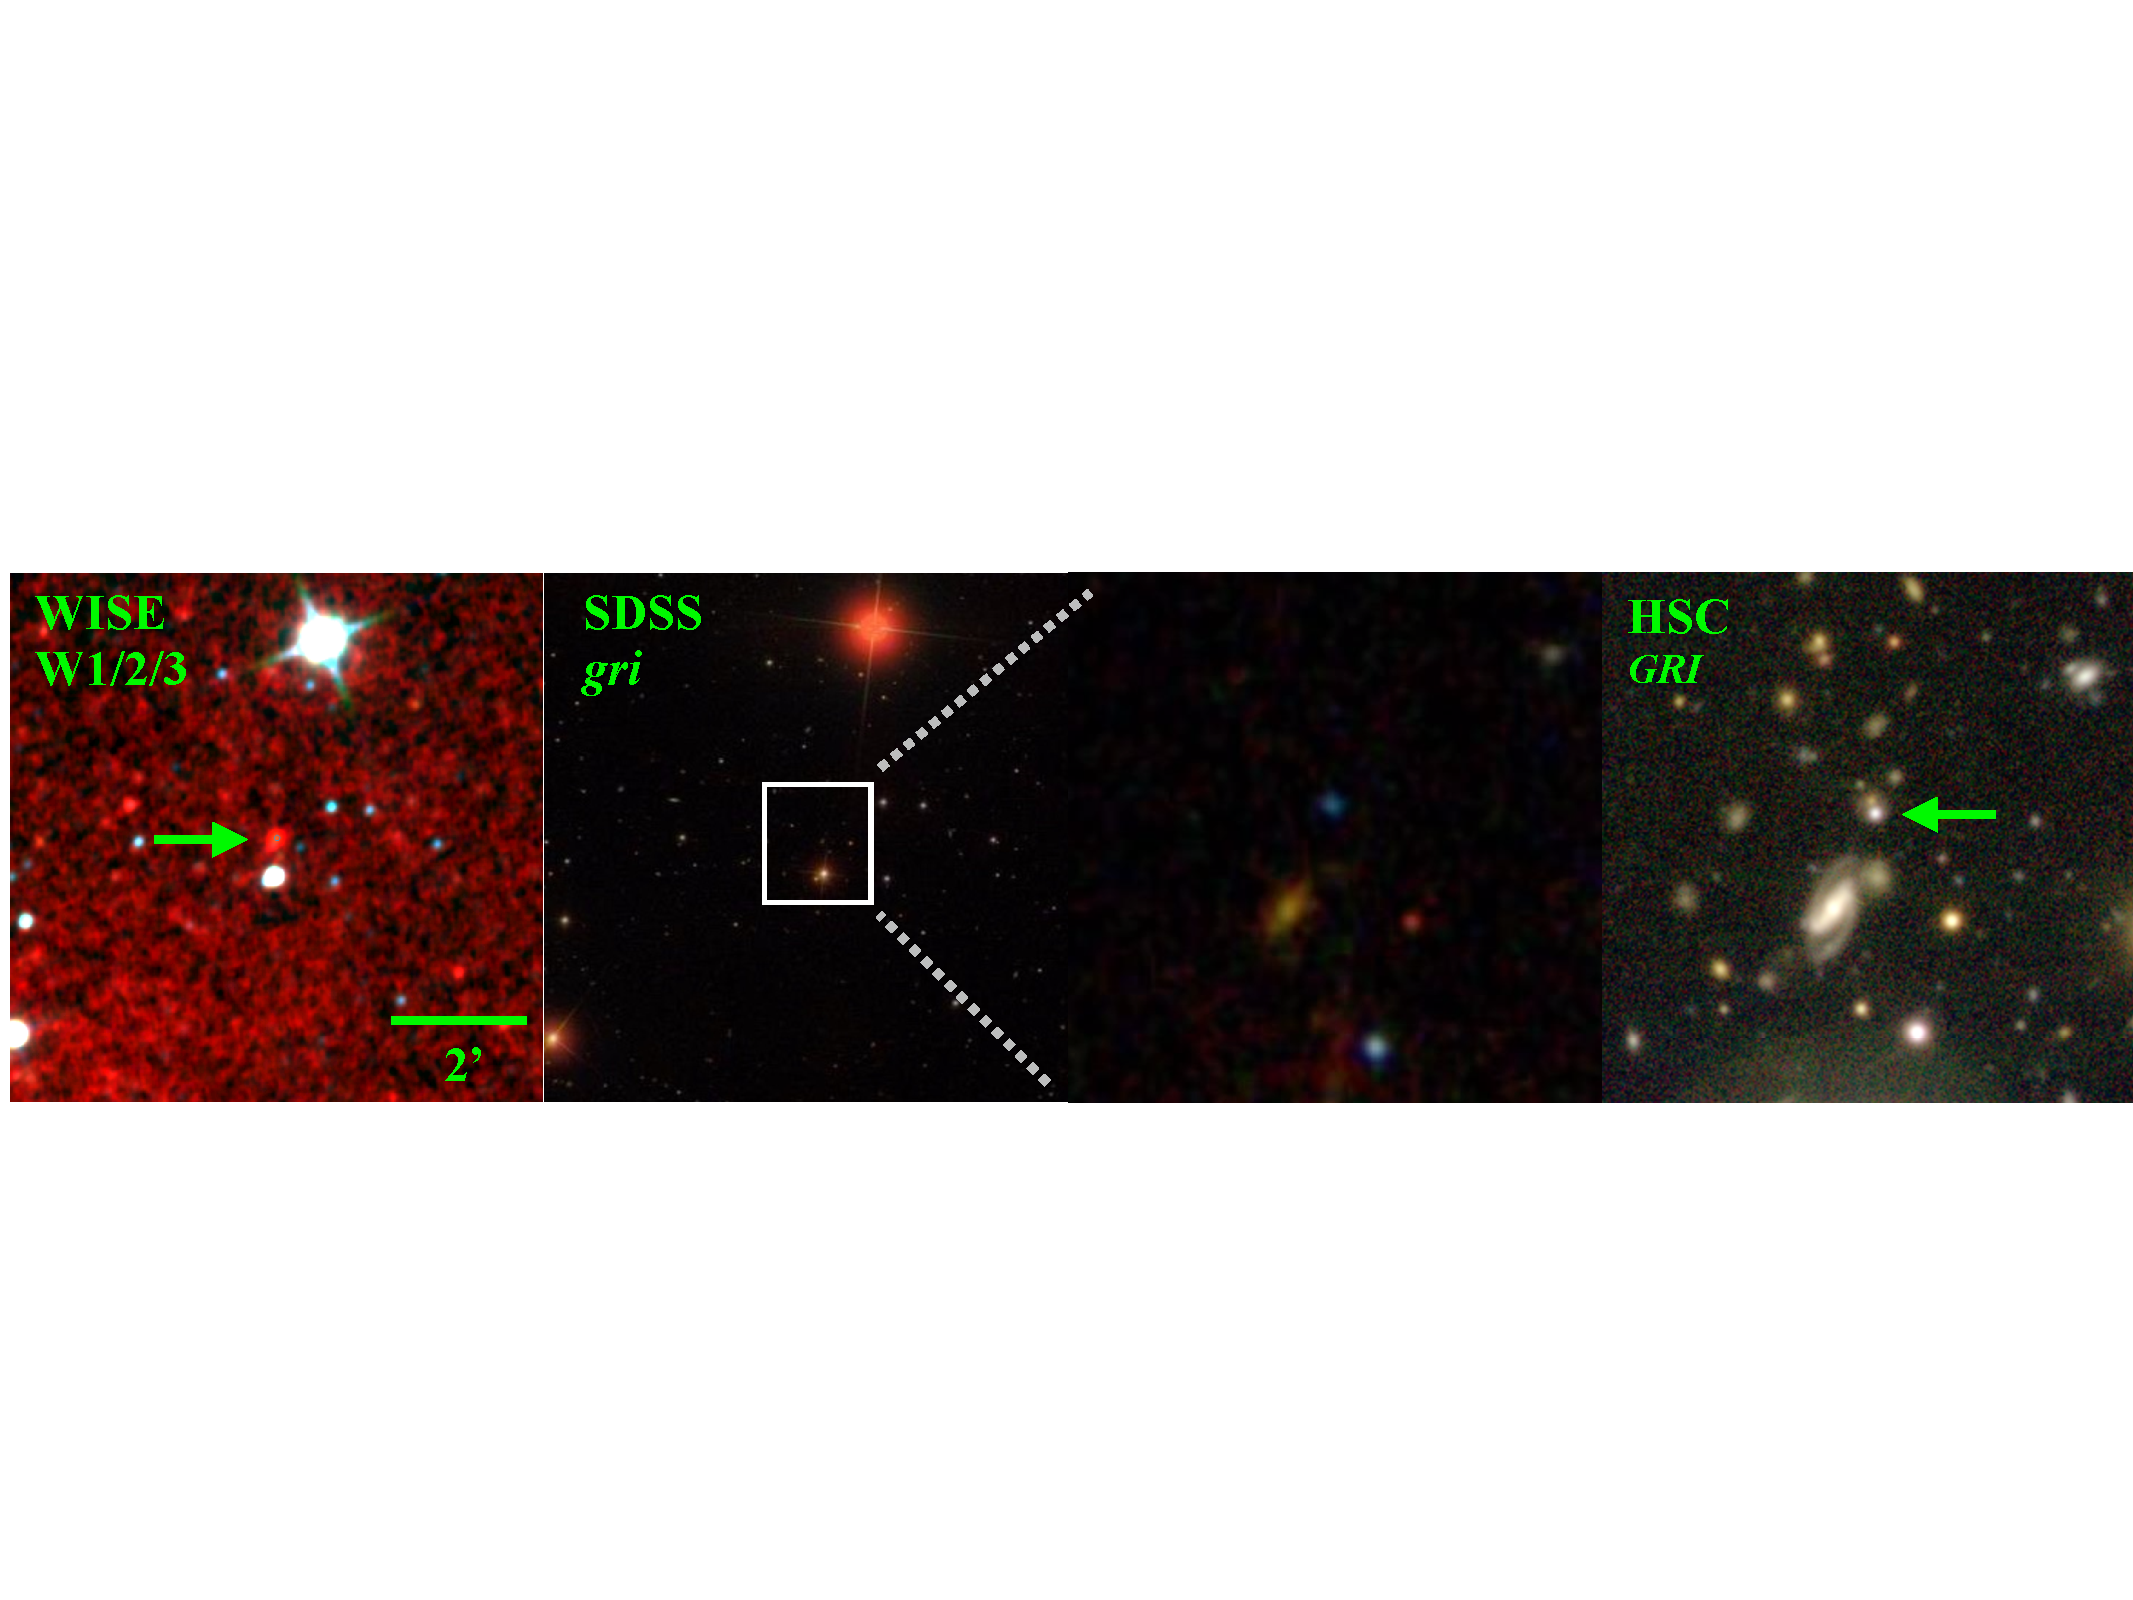
\includegraphics[width=17.0cm, trim={0.15cm 0 0.05cm 0},clip]
   {figures/WISE_SDSSzoomHSC_ERQ-image_v3.pdf}
    \vspace{-20pt}
   \caption{%\small   
\footnotesize 
%     \scriptsize
 %    \tiny
The IR and optical imaging of J2323-0100, an archetype of the
``Extremely Red Quasars'' (ERQs) at $z\approx2.5$ and a {\it JWST}
target. Shown are WISE {\it (left)}, where the quasar booms out as
indicated by the arrow; the SDSS image {\it (middle left)} with
zoom-in {\it (middle right)} on the optically faint source, and new
HSC imaging {\it (right)}, which shows tantalizing evidence for a
faint companion galaxy. Optical rest-frame spectra of J2323-0100,
revealed very broad (FWHM = 2500-5000 km s$^{-1}$), strongly
blue-shifted (by up to 1500 km s$^{-1}$) \oiii\ $\lambda$5007\AA\
emission lines in the ERQs. This is suggestive of active outflows and
potentially evidence for AGN feedback in action at the height of SMBH
activity.
}
  \vspace{-12pt}
 \label{fig:ERQ}
\end{center}
\end{figure}

\medskip
\medskip
\smallskip
\smallskip
\noindent
\textbf{\textsc{WP5: Observations of Quasars by the James Webb Space Telescope}} 

\smallskip
\smallskip
\noindent
In \citet{Ross2015} I discovered a new class of object, the ``extremely red
quasars'', that have optical spectroscopy from SDSS/BOSS, and
$r-[22\mu{\rm m}]>14$ colors (i.e., $F_{\nu,\, {\rm MIR}} / F_{\nu,\,
{\rm opt}} \gtrsim 1000$) from the Wide-field Infrared Survey Explorer
\citep[WISE;][]{Wright2010} satellite, see Figure~\ref{fig:ERQ}.  The ERQs are a
unique obscured quasar population with extreme physical conditions
related to powerful outflows across the line-forming regions. As my team 
have shown, these
sources are the signposts of the most dramatic form of quasar feedback
at the peak epoch of galaxy formation, and may represent an active
``blow-out'' phase of quasar evolution \citep{Zakamska2016, Hamann2017}.  
 However, due to
the current lack of access to mid-infrared spectroscopy, it is still
unknown whether the large IR luminosities observed in these quasars is
from star formation, which would produce strong polycyclic aromatic
hydrocarbon (PAH) spectral features, or, if it is from the hot dust
near the central quasar, which should produce much weaker/no PAH
emission.

\smallskip
\smallskip
\noindent
What are the star-formation properties of luminous quasars at the peak
of quasar activity?  We aim to answer this by looking for the presence
of polycyclic aromatic hydrocarbon (PAH) spectral features in infrared
bright quasars with the {\it James Webb Space Telescope} (JWST).  

\smallskip
\smallskip
\noindent
{\bf WP5 is high risk, high-reward.}  This is an ideal investigation for
the JWST, but we classify this as high-risk since we have to apply for
the telescope time and are not guaranteed the data.  We note this will
be the single WP NPR would lead and does not impact in any direct way
the other WPs. This would lead to very-high gain science.  

\smallskip
\smallskip
\noindent
{\bf Key
Deliverables:} State-of-the-art data products from the JWST, with the
observational evidence and physical interpretation of how ``quasar
feedback'' regulates galaxy formation in high-redshift quasars.
{\bf Timelime:} The deadline for JWST Cycle 1 GO programmes is 
06th April 2018, so I will know if I have been awarded observing 
time here before the start of the ERC. 


%%%
%%%   W P   6 
%%%
\medskip
\medskip
\smallskip
\smallskip
\noindent
\textbf{\textsc{WP6: New Object Discovery:}} 

\smallskip
\smallskip
\noindent
The LSST will scan the sky repeatedly, enabling it, and us, to both
discover new, distant transient events and to study variable objects
throughout our universe. The LSST will extend our view of the
changeable universe a thousand times over current surveys.  The most
interesting science to come may well be the discovery of new classes
of objects.

\smallskip
\smallskip
\noindent
{\bf WP6 is medium-risk, exceptionally high-reward.}  We class this as
medium-risk, since it is tricky to class a WP with essentially unknown
discovery potential as fully `low-risk'. However, we do not classify
this as `high-risk' since if there was a paucity of discovery of novel
classes of objects, this would be the first time in the history of
observational astrophysics that a new facility such as LSST has come
online and found nothing new.  

\smallskip
\smallskip
\noindent
{\bf Key Deliverables:} Potential
discovery of new classes of astronomical objects.
{\bf Timeline:} Peak Discovery Potential will come during the 
very early operation of LSST. We have to thus have {\tt QuasarSieve}, 
our ML light curve algorithms trained, and be ready 
to follow-up where necessary here. 


\medskip  \medskip \smallskip \smallskip \noindent
\subsection{Feasibility}

\smallskip
\smallskip
\noindent
By its inherent nature, our programme is high-risk and high-reward, but
we {\it fundamentally} have the personnel and skill sets that are 
necessary to make this project feasible. 
%% Mention your experience and knowledge to hedge against this risk or alternative approaches or help from collaborators. 
The P.I. has a track-record of managing scientific groups in 
large international and world-leading collaborations. {\it Critically, 
he also has a track record of developing key software packages 
on strict deadlines, e.g. the BOSS Quasar Target Selection software 
package (that contained a suite of novel ML algorithms).}
%
%% Have a dedicated section on feasibility of what you are proposing. Explain which WP’s/tasks present high levels of risk. 
%
%%Provide a contingency plan, particularly if any of the tasks are unconventional, present a great challenge and are high risk (but also high gain). 

%
%% Be ``safely adventurous''.  
%
%% Include a gantt chart or a timeline for the evaluators to visualise the timescale of each component of the work you are proposing.  Include a 4-5 line summary to recap and remind the evaluator what the essence of the project is and why it so important to get this funded now.




